\section{Discussion}
Transforming a time-driven into an event-driven approach should always be possible because the ability to schedule events with timestamps allows to map all features of time-driven ABS to an event-driven one - the discussion above should give a good direction of how this process works. Still for some models one can argue that the time-driven approach is much more expressive than an event-driven one, and we think this is certainly the case for the SIR model. The event-driven approach leads to much more fragmented logical flow and agent behaviour especially in the case of synchronous agent interactions. Still, we have shown a possible direction of reducing the fragmentation using the \textit{tagless final} approach.

\subsection{A related approach}
The work of \cite{botta_time_2010} tries to solve a similar problem. The authors also use Haskell to implement ABS and more specifically looked into the use of messages and the problem of when to advance time in models with arbitrary number synchronised agent-interactions.
The biggest difference is, that we approach our agents fundamentally different through the use of Monads and FRP. First in our approach an agent is only a single MSF and thus can not be directly queried for its internal state / its id or outgoing messages, instead of taking a list of messages, our agents take a single event/message and can produce an arbitrary number of outgoing messages together with an observable state - note that this would allow to query the agent for its id and its state as well by simply sending a corresponding message to the agents MSF and requiring the agent to implement message handling for it. Also the state of our agents is \textit{completely} localised and there is no means of accessing the state from outside the agent, they are thus "fully encapsulated agents" \cite{botta_time_2010}. Note that the authors of \cite{botta_time_2010} define their agents with a polymorphic agent-state type \textit{s}, which implies that without knowledge of the specific type of \textit{s} there would be no way of accessing the state, rendering it in fact also fully encapsulated.
The problem of advancing time in our approach is conceptually very similar though: after sending a tick message to each agent (in random order), we process all agents until they are idle: there are no more enqueued messages / events in the queue. The similarities in both approaches might hint at that this seems to be indeed the "right" way to go. % TODO: can we really say this in a thesis?

\subsection{Layered architecture}
The approach is designed as a 3-layered architecture, see Figure \ref{fig:3layer_system}:
\begin{enumerate}
	\item \textit{Pure functions} are the working horses, which do the actual computations of the simulation. They are mostly used to build up the 2nd layer. Also layer 1 might access them to achieve pure computations when there is no need for effects.
	\item \textit{Monad transformer stack} (global and local) does the dirty work of effectful computation: sending messages, mutating the environment, reading model configuration, drawing random numbers, mutating agent state. This layer uses the pure functions to build up its functionality and also propagates between the 1st and 3rd layer.
	\item \textit{MSFs} (arrowized FRP) are the backbones of the architecture and define the dynamical structure of the system. This layer builds heavily on the 2nd layer and can also be seen as a highly delegation mechanism. Note that MSFs blur the distinctions between the monadic and the arrowized layer.
\end{enumerate}

\begin{figure}
	\centering
	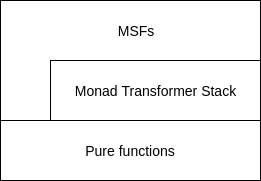
\includegraphics[width=.4\textwidth, angle=0]{./fig/eventdriven/3layers.png}
	\caption{The architecture as a 3-layered system.}
	\label{fig:3layer_system}
\end{figure}

Separating those 3 concerns from each other makes the code more robust, easier to refactor and maintain. Further it makes code \textit{much} easier to test as will be shown in Chapter \ref{ch:property}. 

% maybe refactor sugarscape: write more pure functions which make the distinction between read only and write only of the agent state clear e.g. is agent fertile can be a pure function with state passed explicitly. also always make clear that we can write functions which are monadic but access e.g. only the agent state or the Environment state Without the full monad Transformer stack: try to refactor more in this direction and make thus very clear in the discussion

\subsection{Imperative nature}
Both event-driven use-cases (Sugarscape and SIR) makes heavy use of the State Monad, thus one might ask what the benefits are of our pure functional approach - after all we seem to fall back into stateful, imperative style programming. %We agree that our approach is just one way of implementing ABS in FP but we think we have come a long way thus making our approach quite valuable even if there might be other approaches like shallow EDSLs or freer monads (see Chapter \ref{sec:alternatives}).
On the other hand even our stateful programming is highly restricted to very specific types and operations. Further, in our monad stack we control the operations possible to the respective layers: e.g. sending messages/events is a write-only operation (as it should be), accessing the unique agent-id and the model-configuration is read-only (as it should be). All this is guaranteed at compile time, which makes it much more manageable, maintainable, robust, composable and testable.
To quote John Carmack \footnote{\url{http://www.gamasutra.com/view/news/169296/Indepth_Functional_programming_in_C.php}}: \emph{"A large fraction of the flaws in software development are due to programmers not fully understanding all the possible states their code may execute in."}. We claim that despite using an imperative style, the static guarantees of the types we operate on and the operations provided, it makes it easier to fully understand the possible states of the simulation code.

%\subsection{Lines of code}
%TODO: report LoC and compare it with other implementations we found on the internet

\subsection{Multiple types of agents}
In the Sugarscape example we have only considered one type of agents, thus the whole population is a homogeneous one in regards of the \textit{type} of the agent. It is quite straightforward to have heterogeneous agent types as well, which is accomplished through adding additional data-declarations to the observable output and the agent-state. A consequence is that all agent types have to speak the same event-language because in regards of types the agents are treated the same way - this is also true for the monadic / effect stack: different agent types cannot have different effect types in this approach as they are seen as the same on the type level.

\subsection{Performance}
The event-driven implementation from this Chapter is around 60 - 70\% faster than the time-driven implementation from Chapter \ref{sec:timedriven_firststep}, which is non-monadic and uses the FRP library Yampa. For the monadic time-driven approach of Chapter \ref{sec:adding_env} the difference is much more dramatic: it is about 700 - 800\% slower. These results dramatically highlight the problem of time-driven ABS: its performance cannot compete with an even-driven approach. This is exaggerated even more so when making use of MSFs as in Chapter \ref{sec:adding_env}. In this case, a time-driven approach becomes extremely expensive in terms of performance and one should consider an event-driven approach. In case the model is specified in a time-driven way, a transformation into an event-driven approach should always be possible as outlined above.

We compared an event-driven SIR implementation we did in Java to the Haskell one here. We run for 150 time steps with 1,000 susceptible and 1 infected agent, $\beta = 5$, $\gamma = 0.05$, $\delta = 15$. Further, we fixed the random-number generators to guarantee identical dynamics in every run and averaged 8 runs. The Java implementation averages at 1.2 seconds, whereas the Haskell implementation at 6.8 seconds. These performance figures are closer than the ones in the time-driven approach of the previous chapter. This shows that event-driven is indeed much better performing and also more flexible as \cite{meyer_event-driven_2014} has pointed out. Interestingly, the time-driven Java implementation outperforms the event-driven one. Although, we have improved the performance substantially compared to the time-driven approach, we address it more in-depth in the chapters on parallelism \ref{ch:parallelism_ABS} and concurrency \ref{ch:concurrent_abs}.

% EVENT-DRIVEN
% Java: 1262, 1259, 1159, 1202, 1182, 1152, 1238, 1238 Milliseconds
% Haskell: 6.8, 6.6, 6.3, 6.3, 6.5, 6.3, 6.3, 6.8 Seconds

\subsection{Conclusion}
Overall we think that this event-driven approach is quite feasible and is \textit{the way to go} to implement ABS in a pure functional way. The time-driven approach is quite expressive but is not as flexible and general as the event-driven one. Also performance is considerably better in event-driven approach.

We conclude that synchronous agent-interaction was the most difficult part to figure out and get right and thus posed the greatest challenge. This concept is indeed cumbersome and clearly more complex than direct method invocation in object-oriented programming. Unfortunately, with the goal of staying pure we do not have much other options. Note, that we didn't aim to encapsulate its complexity behind domain-specific combinators but this is certainly possible and should reduce the difficulty and complexity considerably. This is left as further research and open work which should be untertaken in the future, when putting all the concepts of this thesis into a general purpose library for pure functional ABS in Haskell.

% direct MSF call, Problem is recursive nature. maybe try it with gintis Implementation. I just learned that what i want to achieve is actually: https://en.wikipedia.org/wiki/This_(computer_programming)#Open_recursion AND OPEN RECURSION IS PRETTY BAD